\section{Implementation}

In this section the author discusses the implementation of the experimental system to prove the concept of the proposed load balancers with ECMP redundancy in detail.

\subsection{Experimental system architecture}\label{sec:poc}

\begin{figure}[h]
\centering
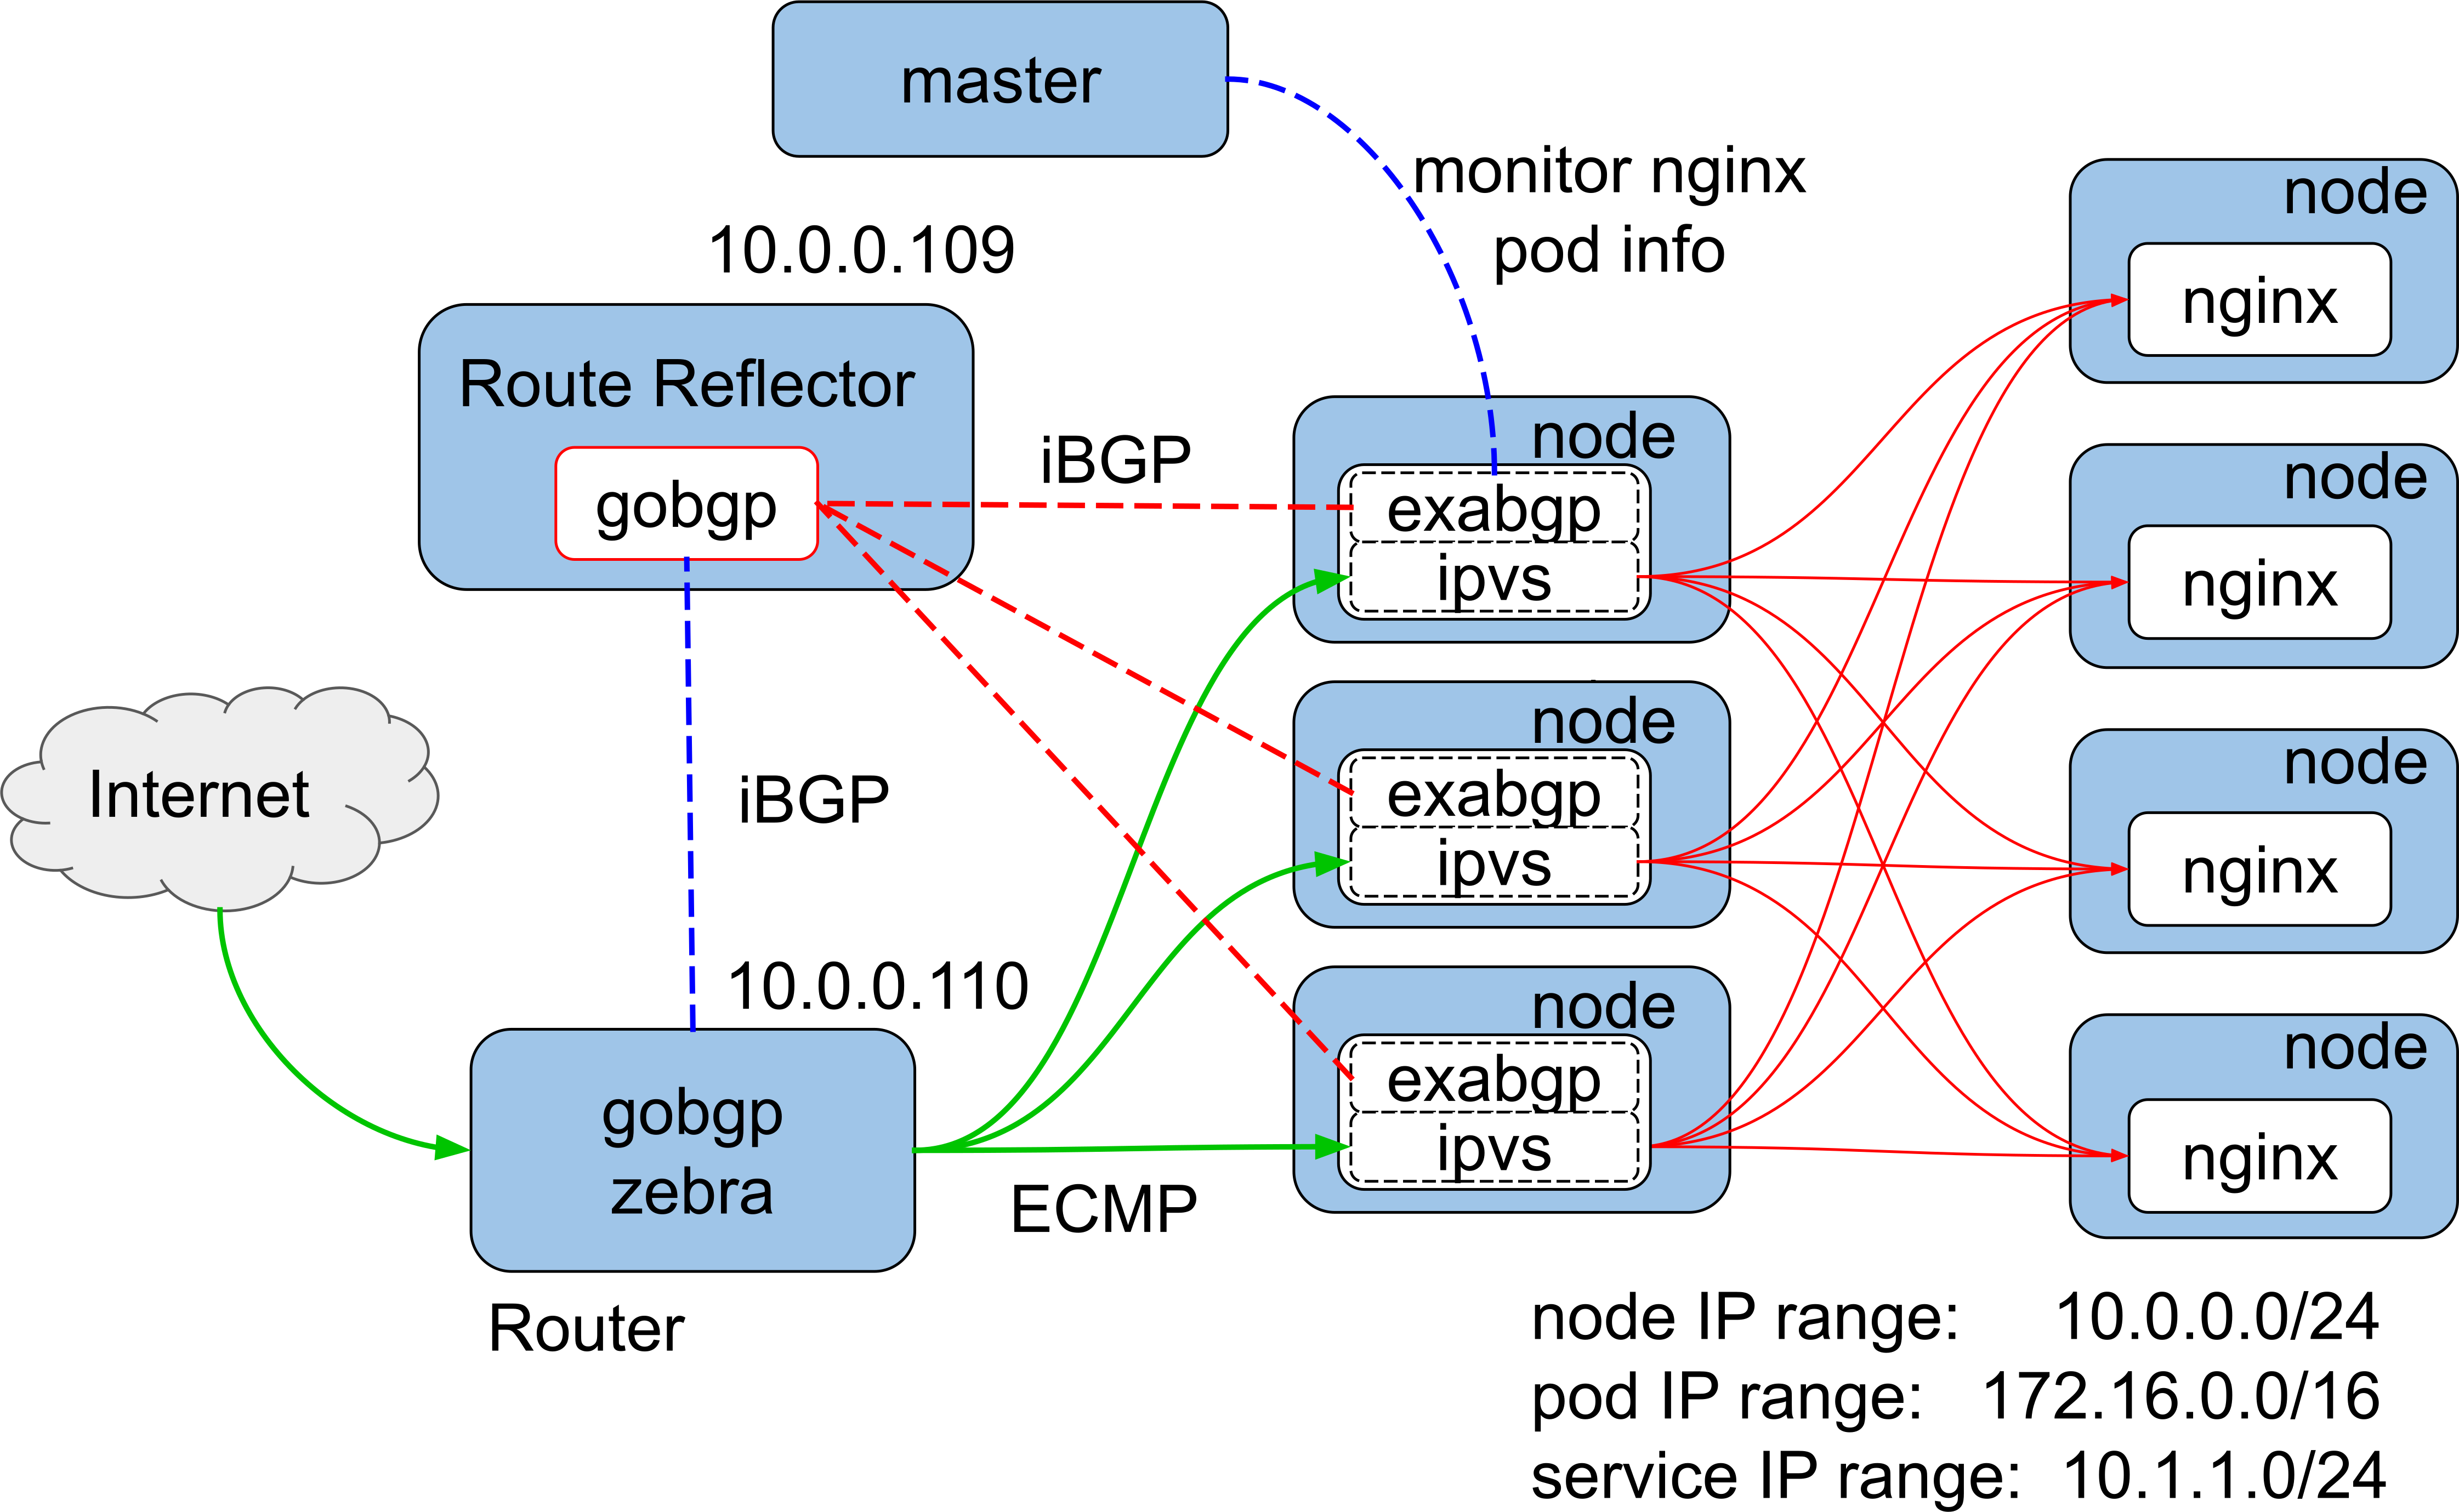
\includegraphics[width=0.9\columnwidth]{Figs/poc.png}

\par\bigskip
\centering
\begin{minipage}{0.9\columnwidth}
  \caption[Container cluster with proposed redundant software balancers]{
    An experimental container cluster with proposed redundant software balancers.
    The master and nodes are configured as Kubernetes's master and nodes on top of conventional Linux systems, respectively.
    The route reflector and the upstream router are also conventional Linux systems.
    For the green lines, a service IP address is used. The red lines use the IP addresses of the overlay network. The blue line uses the IP addresses of the node network.
  }
  \label{fig:poc}
\end{minipage}

\end{figure}

Figure~\ref{fig:poc} shows the schematic diagram of proof of concept container cluster system with the proposed software load balancers.
%
Each load balancer pod consists of an exabgp \cite{exa-networks_2018} container and an IPVS container.
The IPVS container is responsible for distributing the traffic toward the service IP to web server (nginx) pods.
The IP address for nginx pods and load balancer pods are dynamically assigned upon launch of themselves from 172.16.0.0/16 address range.
The IPVS container monitors the availability of web server pods by consulting apiserver on the master node and manages the load balancing rule appropriately.
The exabgp container is responsible for advertising the route toward the service IP to the route reflector using BGP.
The route reflector aggregates the routing information advertised by load balancer pods and advertise them to the upstream router.
The upstream router updates its routing table according to the advertisement.

All the nodes and route reflector are configured using Debian 9.5 with self compiled linux-4.16.12 kernel.  
The author also used conventional Linux system as an upstream router for testing purpose, using the same OS as the nodes and the route reflector.
The version of Linux kernel needed to be 4.12 or later to support hash based ECMP routing table.
The author also needed to enable kernel config option CONFIG\_IP\_ROUTE\_MULTIPATH \cite{ipsysctl} when compiling, and set the kernel parameter fib\_multipath\_hash\_policy=1 at run time.
Although in the actual production environment proprietary hardware router with the highest throughput is usually deployed, one can still test some of the advanced features by using a conventional Linux system for the upstream router.

\begin{table}[h]
  \centering
  \begin{tabular}{|l|c|c|c|}
    \hline
    \begin{tabular}{l} Features \end{tabular} & \multicolumn{1}{c|}{gobgpd} & \multicolumn{1}{c|}{exabgp} & \multicolumn{1}{c|}{bird} \\ \hline
    \begin{tabular}{l} Static route advertisement \end{tabular} & complex & simple & complex  \\ \hline
    \begin{tabular}{l} Add-path support$^{*}$ \end{tabular} & Yes & No & Yes  \\ \hline
    \begin{tabular}{l} Dynamic neighbor$^{**}$ \end{tabular} & Yes & No & No \\ \hline
    \begin{tabular}{l} FIB manipulation \end{tabular} & Yes (through zebra) & No & Yes (Native) \\ \hline
%    \begin{tabular}{l} Use case \end{tabular} & Router/Route reflector & Load balancer & Not used$^{**}$  \\ \hline
  \end{tabular}

  \par\bigskip
  \centering
  \begin{minipage}{0.9\columnwidth}
    \caption[Comparison of open source BGP agents]{
      Comparison of open source BGP agents.
      Open source BGP agents are compared in terms of the features required in the proposed systems. \par
      \small
      $^{*}$ \phantom{$^{*}$} The add-path is the feature to support multipath advertisement. \par
      $^{**}$ \phantom{$^{}$} The dynamic-neighbor is the feature to describe peer group as a range of IP address.
    }
    \label{table:bgp_agents}
  \end{minipage}
\end{table}

Table~\ref{table:bgp_agents} compares open source BGP agents in terms of required features for the proposed architecture.
Each load balancer {\em pod} needs to advertise itself as the next hop for packets toward the service IP.
For that purpose, exabgp is preferable because it only requires to add a line, e.g., \enquote{route [Service\_IP] next-hop [Pod\_IP]} in the configuration file.
On the other hand, the gobgpd and the bird require other client programs to inject the static route after the daemon itself is up and running.
For example, in the case of gobgpd, after launching gobgpd, a user is required to issue a command line, e.g., \enquote{gobgp global rib add [Service\_IP]/32 origin igp nexthop [Pod\_IP] community 100:50 -a ipv4}.
 (The gobgp is a client program to manage gobgpd.)
This is a bit complex and error-prone, especially when one has to inject the route periodically inside a container.

As for the route reflector, add-path \cite{rfc7911} feature and dynamic neighbor feature are needed. These are supported by gobgpd.
For the upstream router Forwarding Information Base (FIB) manipulation \cite{exa-networks_2018} feature is needed, which is supported by gobgpd through zebra \cite{jakma2014introduction,osrg_gobgp_zebra}.
As a result, exabgp is used for the load balancer pods, gobgpd is used for the route reflector, and gobgpd and zebra are used for the upstream router.


The other requirement for the route reflector is the knowledge of the overlay network for the containers.
The configurations for the upstream router is summarised in Appendix~\ref{appendix:router_config}.
The configurations for the route reflector is summarised in Appendix~\ref{appendix:route_reflector_config}.

\subsection{IPVS container}\label{sec:ipvs}

In order to implement a software load balancer that is runnable in any environment, the author used Linux kernel's IPVS in Docker container.
In addition to that, the proposed load balancer uses two other components, keepalived{, and a }controller.
These components are placed in a single Docker container image.
\deleted[id=4th]{The Dockerfile, a shell script file and the template files used to create the load balancer container are shown in Appendix~\ref{appendix:ipvs_container}. }
The IPVS is a Layer-4 load balancer capability, which is included in the Linux kernel 2.6.0 released in 2003 or later,
to distribute incoming Transmission Control Protocol (TCP) traffic to
{\em real servers}\footnote{The term, {\em real servers} refers to worker servers that will respond to incoming traffic,
in the original literature \cite{Zhang2000}. The author will also use this term in a similar way.} \cite{Zhang2000}.
For example, IPVS distributes incoming Hypertext Transfer Protocol (HTTP) traffic destined for a single destination IP address,
to multiple HTTP servers (e.g. Apache HTTP or nginx) running on multiple nodes in order to improve the performance of web services.
Keepalived is a management program that performs health checking for {\em real servers}
and manages IPVS balancing rules in the kernel accordingly.
It is often used together with IPVS to facilitate ease of use.
The controller is a daemon that periodically monitors the {\em pod} information on the master,
and it performs various actions when such information changes.
Kubernetes provides ingress controller framework as the Go Language (Golang) package to implement the controllers.
The author implemented a controller program that feeds {\em pod} state changes to keepalived
using this framework (Appendix~\ref{appendix:ingress_controller}).

\begin{figure}[h]
  \centering
  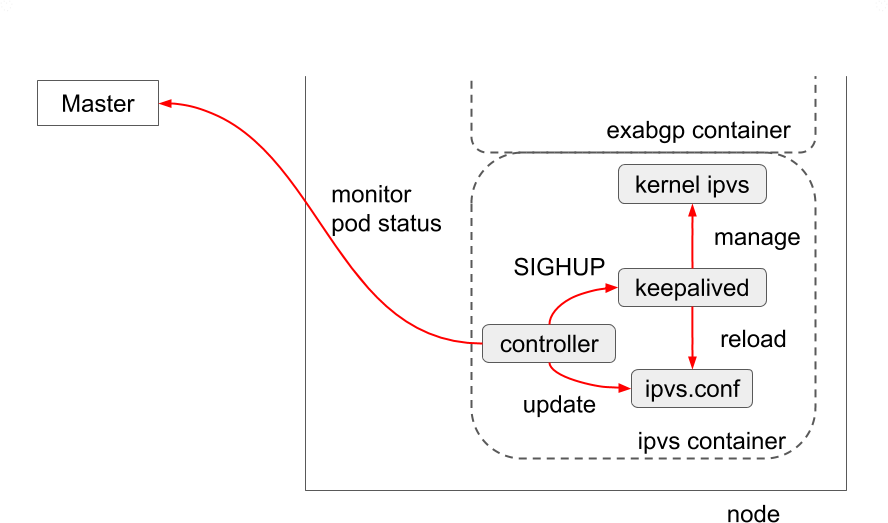
\includegraphics[width=0.9\columnwidth]{Figs/ipvs-ingress-schem}
  
    \par\bigskip
    \centering
    \begin{minipage}{0.9\columnwidth}
      \caption[Implementation of IPVS container]{
        Implementation of IPVS container.
        The controller checks the pod status every second, by consulting the master node.
        Upon a change of the status, the controller updates the ipvs.conf and sends SIGHUP to keepalived.
        The keepalived reload the ipvs.conf and updates the load balancing rules in the kernel correctly.
      }
      \label{fig:ipvs-ingress-schem}
    \end{minipage}
\end{figure}

The proposed load balancer needs to dynamically reconfigure the IPVS balancing rules whenever {\em pods} are created or deleted. 
Figure~\ref{fig:ipvs-ingress-schem} is a schematic diagram of IPVS container to show the dynamic reconfiguration of the IPVS rules.
Two daemon programs, controller and keepalived, running in the container are illustrated.
The keepalived manages Linux kernel's IPVS rules depending on the ipvs.conf configuration file.
It can also periodically check the liveness of a {\em real server}, which is represented as a combination of the IP addresses and port numbers of the target {\em pods}. 
If the health check to a {\em real server} fails, keepalived will remove that {\em real server} from the IPVS rules immediately.
The interval of the health check is typically 1 to several seconds and is arbitrarily determined by users.  

Every second, the controller monitors information concerning the running {\em pods} of a web application in the Kubernetes cluster by consulting the apiserver running in the master through its API.
Whenever {\em pods} are created or deleted, the controller notices the change and automatically regenerate an appropriate ipvs.conf 
and issue SIGHUP to keepalived within a second.
Then, keepalived will reload the ipvs.conf, and modify the IPVS rules inside the kernel appropriately depending on the result of the health check.

When a pod is terminated, existing connections are reset by the node kernel.
The SYN packets sent to a pod after termination, but before the IPVS rule update, will be answered with ICMP unreachable by the node.
In these cases, the client sees connection errors.
However, since the load balancer rule update is within a second, these errors can be regarded as the tolerable rare exceptions.
In order to avoid the connection errors to be seen by a human, HTTP client programs are required to re-initiate the connection.

The actual controller \cite{ktaka_ccmp_2017_826894} is implemented using the Kubernetes ingress controller \cite{K8sIngress2017} framework. 
By importing existing Golang package, \enquote{k8s.io/ingress/core/pkg/ingress}, the author could simplify the implementation, e.g. 
120 lines of code (Appendix~\ref{appendix:ingress_controller}).
%
Keepalived and the controller are placed in the docker image of IPVS container.
The namespace separation for IPVS has already been supported in the recent Linux kernel. 

Configurations for capabilities were needed when deploying the IPVS container: adding the CAP\_SYS\_MODULE capability 
to the container to allow the kernel to load required kernel modules inside a container, 
and adding CAP\_NET\_ADMIN capability to the container to allow keepalived to manipulate the kernel's IPVS rules. 
For the former case, the author also needed to mount the \enquote{/lib/module} of the node's file system on the container's file system.

\begin{figure}[h]
  \centering
  \begin{minipage}{0.6\columnwidth}
    \begin{lstlisting}[frame=lines,breaklines=true,basicstyle=\small\ttfamily]
      virtual_server fwmark 1 {
        delay_loop 5
        lb_algo lc
        lb_kind NAT
        protocol TCP
        real_server 172.16.21.2 80 {
          uthreshold 20000
          TCP_CHECK {
            connect_timeout 5
        connect_port 80
          }
        }
        real_server 172.16.80.2 80 {
          uthreshold 20000
          TCP_CHECK {
            connect_timeout 5
            connect_port 80
          }
        }
      }
    \end{lstlisting}
  \end{minipage}

  \par\bigskip
    \centering
    \begin{minipage}{0.9\columnwidth}
      \caption[An example of ipvs.conf]{
        An example of ipvs.conf
        This configuration file is auto-generated by the controller.
        The controller periodically accesses the apiserver on the master node and constantly monitor the status of running pods.
      }
      \label{fig:ipvs.conf}
    \end{minipage}
\end{figure}

\begin{figure}[h]
  \centering
  \begin{minipage}{0.95\columnwidth}
   \begin{lstlisting}[frame=lines,breaklines=true,basicstyle=\small\ttfamily]
 IP Virtual Server version 1.2.1 (size=4096)
 Prot LocalAddress:Port Scheduler Flags
  -> RemoteAddress:Port Forward Weight ActiveConn InActConn
 FWM  1 lc
  -> 172.16.21.2:80      Masq    1      0          0         
  -> 172.16.80.2:80      Masq    1      0          0
   \end{lstlisting}
  \end{minipage}

  \par\bigskip
  \centering
  \begin{minipage}{0.9\columnwidth}
    \caption[Example of IPVS balancing rules]{
      Example of IPVS balancing rules.
      This shows the load balancing rule in a load balancer container.
      The packet that has FWM (fwmark)=1 will be forwarded to two real servers using the least connection (lc) balancing algorithm.
      The fwmark is a parameter that is only available inside a socket buffer in Linux kernel.
      The fwmark can be put and manipulated by the iptables program, once a socket buffer for a received packet is assigned by the kernel.
      }
    \label{fig:IPVS rule}
  \end{minipage}
\end{figure}

Figure~\ref{fig:ipvs.conf} and Figure~\ref{fig:IPVS rule} show an example of an ipvs.conf file 
generated by the controller and the corresponding IPVS load balancing rules, respectively.
Here, we can see that the packet with {\tt fwmark=1} \cite{BertHubert2002} is distributed 
to {\em 172.16.21.2:80} and {\em 172.16.80.2:80} using the masquerade mode (Masq) and the least connection (lc) \cite{Zhang2000} balancing algorithm.

\FloatBarrier

\begin{figure}[h]
  \centering
  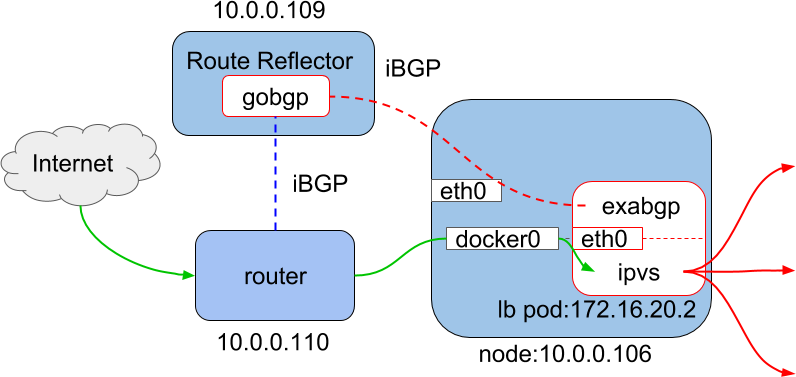
\includegraphics[width=0.9\columnwidth]{Figs/exabgp}
  
  \par\bigskip
  \centering
  \begin{minipage}{0.9\columnwidth}
    \caption[Network path by the exabgp container]{
      Network path by the exabgp container.
      The packets from Internet to service IPs, 10.1.1.0/24 are routed to the load balancer pod (green arrows) by the set of routing rules shown in Table~\ref{table:exabgp_setting}.
      And then the IPVS container forwards them to nginx pods (red arrows).
      The IP address of any pod is dynamically assigned from 172.16.0.0/16 when the pod is started. 
    }
    \label{fig:exabgp_schem}
  \end{minipage}

\end{figure}

\subsection{BGP software container}\label{sec:bgp}

\begin{table}

  \centering
  \begin{minipage}{0.85\columnwidth}
    \begin{lstlisting}[frame=lines,breaklines=true,basicstyle=\small\ttfamily]
 [BGP announcement]
    route 10.1.1.0/24 next-hop 10.0.0.106       ...(1)
 [Routing in node net namespace]
    ip netns exec node \
       ip route replace 10.1.1.0/24 dev docker0 ...(2)
 [Accept as local]
    ip route add local 10.1.1.0/24 dev eth0     ...(3)
    \end{lstlisting}
  \end{minipage}

  \par\bigskip
  \centering
  \begin{minipage}{0.9\columnwidth}
    \caption[Required settings in the exabgp container]{
      Required settings in the exabgp container.
      (1) The node IP address, 10.0.0.106 is used as next-hop for the service IPs, 10.1.1.0/24, in BGP announcement.
      (2) In order to route the packets destined toward the service IP to the container, a routing rule to the dev docker0 is created in the node net namespace. 
      (3) A routing rule to accept the packets destined toward the service IPs,  as local is also required.
    }
    \label{table:exabgp_setting}
  \end{minipage}

\end{table}

In order to implement the ECMP redundancy, the author also containerized exabgp using Docker.
\deleted[id=4th]{The Dockerfile and a shell script file used to create the BGP software container are shown in Appendix~\ref{appendix:exabgp_container}. }
Figure~\ref{fig:exabgp_schem} shows a schematic diagram of the network path realized by the exabgp container.
As mentioned earlier, the author used exabgp as the BGP advertiser. 
The ingress traffic from the Internet is forwarded by ECMP routing table on the router to the node that hosts a load balancer pod.
And then it is routed to the load balancer pod according to the set of routing rules in Table~\ref{table:exabgp_setting}(2),(3).
After that the IPVS forwards them to nginx pods.
The IP address of any pod is dynamically assigned from 172.16.0.0/16 when the pod is started. 

Table~\ref{table:exabgp_setting} summarises some key settings required in the exabgp container to route the traffic to the IPVS container.
(1) In BGP announcements the node IP address, 10.0.0.106 is used as the next-hop for the service IPs, 10.1.1.0/24.
(2) Then on the node, in order to route the packets toward the service IPs to the IPVS container, 
a routing rule for 10.1.1.0/24 to the dev docker0 is created in the node net namespace. 
(3) A routing rule to accept the packets toward the service IPs as local is also required in the container net namespace. 
The configuration for exabgp is shown in Appendix~\ref{appendix:exabgp_config}.

\FloatBarrier

\section{Summary}

In this chapter, the author provided a discussion of load balancer architecture and its implementations suitable for container clusters.
%
First, the author discussed the problems of conventional architecture.
Since Kubernetes is dependent on external load balancers provided by the cloud infrastructures,
it failed to provide portability of a web application in environments where there was no supported load balancer.
Furthermore, the routes that ingress traffic from the internet follow were very complex and inefficient.

In order to alleviate these problems, the author proposed a cluster of software load balancers in containers.
The proposed load balancers utilized container technology and were managed by Kubernetes.
As a result, it is runnable on any environment including cloud infrastructures and on-premise data centers.
Furthermore, since Kubernetes manages load balancer containers, it can quickly scale the number of containers depending on the demand.
%
The author also discussed redundant architecture using ECMP with BGP for proposed load balancer containers.
By using the ECMP, the upstream router can route the ingress traffic to a cluster of load balancer containers in a redundant and scalable manner.
By using BGP, ECMP routing rules in the upstream router are automatically populated, upon the launch of load balancer containers.
The BGP and ECMP are both standard protocols supported by most of the commercial router products.

Thanks to the proposed load balancer, users become being able to set up routes to their web applications automatically, upon its launch, regardless of the infrastructures they use.  
This will greatly improve the portability of a web application and thereby enables migrations.




